\section{Zielsetzung}
    Bei diesem Versuch ist der gedämpte Schwingkreis zu untersuchen. Dabei wird zunächst die Zeitabhängigkeit der Amplitude sowie
    der Widerdstand des aperiodischen Grenzfalles bestimmt. Anschließend wird die Frequenzabhängigkeit der Amplitude der Kondensatorspannung
    und der Phasenverschiebung zwischen Kondensator - und Erregerspannung bei angeschlossener periodischer Spannung untersucht.
\section{Theorie}
    \label{sec:Theorie}
    \subsection{Gedämpfte Schwingungen}
        \begin{figure}
            \centering
            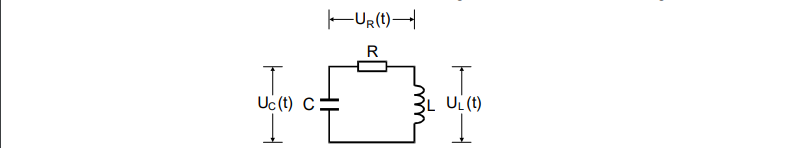
\includegraphics[width=\textwidth]{content/theorie.png}
            \caption{Schematische Darstellung eines gedämpften Schwingkreises\cite[284]{V354}.}
            \label{fig:theorie}
        \end{figure} 
        Bei einem Schwingkreis, bestehend aus einem Kondensator der Kapizät $C$, einer Spule mit der Induktivität $L$
        und einem Dämpfungswiderstand $R$ (siehe \autoref{fig:theorie}) kommt es, bei vorhandener Ladung im Schwingkreis, zu gedämpften 
        Schwingungen. Nach dem zweiten Kirchhoff'schen Gesetz folgt für den vorhandenen Aufbau wie in \autoref{fig:theorie}
        \begin{equation}
            \label{eqn:kirchhoff}
            U_R(t) + U_C(t) + U_L(t) = 0.
        \end{equation}
        Hieraus lässt sich mittels der Beziehungen
        \\ \\
        \centerline{$U_R(t) = R \cdot I(t)$,}
        \centerline{$U_C(t) = \frac{Q(t)}{C}$, wobei $I = \frac{d \, Q}{d \, t}$,}
        und
        \\ \\
        \centerline{$U_L(t) = L \cdot \frac {d \, I} {d \, t} $}
        \\ \\
        die Differentialgleichung 
        \begin{equation}
            \label{eqn:diffgleichung}
            \frac{d^2 \, I}{d \, t^2} + \frac{R}{L} \frac{d \, I}{d \, t} + \frac {1}{L C} = 0
        \end{equation}
        herleiten. Beim Lösen müssen zwei Fälle unterschieden werden, eine reelle, sowie eine imaginäre Lösung. 
        Lösen der Differentialgleichung ergibt im Allgemeinen
        \begin{equation}
            \label{eqn:strom_allgemein}
            I(t) = e^{-2 \pi \mu t} (U_1 e^{i 2 \pi \nu t} + U_2 e^{-i 2 \pi \nu t}),
        \end{equation}
        wobei $\mu = \frac{R}{4 \pi L} $ und $\nu = \frac{1}{2 \pi} \sqrt{\frac{1}{L C} - \frac{R^2}{4 L^2} }$
        substituiert wird.
        \subsubsection{Reelle Lösung - Schwingfall}
            Für den Fall, dass
            \begin{equation}
                \label{eqn:bedingung_reell}
                \frac{1}{L C} > \frac{R^2}{4 L^2}
            \end{equation}
            ist, ist die Lösung reell und damit ergibt sich eine gedämpfte, oszilatorische Schwingung, die sich als
            \begin{equation}
                \label{eqn:reell_lösung}
                I(t) = A_0 e^{-2 \pi \mu t} \cos(2 \pi \nu t + \eta)
            \end{equation}
            darstellen lässt. Dabei beschreibt die Exponentialfunktion die Einhüllende, während die Kosinusfunktion die Schwingung darstellt.
            Deweiteren kann die Abklingdauer $T_ex$ als das Zeitinverall, nachdem die Amplitude der Schwingung auf den $\frac{1}{e}$-ten Teil
            von der Ausgangsamplitude abgesunken ist, zu
            \begin{equation}
                \label{eqn:abklingdauer}
                T_\text{ex} = \frac{1}{2 \pi \mu} = \frac{2 L}{R}
            \end{equation}
            definiert werden.

        \subsubsection{Imaginäre Lösung - Aperiodische Dämpfung}    
            Wenn
            \begin{equation}
                \label{eqn:bedingung_imaginär}
                \frac{1}{L C} > \frac{R^2}{4 L^2}
            \end{equation}
            gilt, ist $\nu$ imaginär.
            Diese Lösung weist keine oszilatorischen Anteile mehr auf und somit treten auch keine Schwingungen mehr auf. Die Lösung
            $I(t)$ kann zunächst einen Extremwert erreichen oder sofort monoton gegen $0$ konvergieren.
            Nach hinreichend großer Zeit gilt
            \begin{equation}
                \label{eqn:imag_lösung}
                I(t) \propto e^{-\Bigl(\frac{R}{2 L} - \sqrt{\frac{R^2}{4 L^2} - \frac {1}{L C}}\Bigr) t},
            \end{equation}
            womit nur noch ein einfaches Relaxationsverhalten vorliegt.
        
        \subsubsection{Aperiodischer Grenzfall}
            Im aperiodischen Grenzfall gilt
            \begin{equation}
                \label{eqn:bedingung_aperiodischerGrenzfall}
                \frac{1}{L C} = \frac {R_\text{ap}^2} {4 L^2},
            \end{equation}
            was dazu führt, dass $\nu = 0$.
            Der aperiodische Grenzfall beschreibt den Fall, bei dem $I(t)$ ohne Überschwingungen am schnellsten gegen $0$ geht.

    \subsection{Erzwungene Schwingungen}        
        Durch anlegen einer äußeren periodischen Spannung $U_\text{err} = U_0 e^{i \omega t }$ ergibt sich die Differentialgleichung \eqref{eqn:diffgleichung}
        zu
        \begin{equation}
            \label{eqn:diffgleichung2}
            \frac{d^2 \, I}{d \, t^2} + \frac{R}{L} \frac{d \, I}{d \, t} + \frac {1}{L C} = U_0 e^{i \omega t}.
        \end{equation}    
        Lösen dieser Differentialgleichung ergibt für die Amplitude $A(t)$ der Kondensatorspannung
        \begin{equation}
            \label{eqn:amplitude}
            A(t) = \frac{U_0 (1 - L C \omega^2 - i \omega R C)}{(1 - L C \omega^2)^2 + \omega^2 R^2 C^2}.
        \end{equation}
        Die Phasenverschiebung $\phi$ zwischen Erregerspannung und Kondensatorspannung ergibt sich zu
        \begin{equation}
            \label{eqn:phasenverschiebung}
            \phi = \arctan \Bigl( \frac {- \omega R C} {1 - L C \omega^2} \Bigr).
        \end{equation}
        Die Kondensatorspannung kann auch in Abhängigkeit von der Winkelgeschwindigkeit $\omega$ angegeben werden zu
        \begin{equation}
            \label{eqn:Kondensatorspannung}
            U_C(\omega) = \frac {U_0} {(1 - L C \omega^2)^2 + \omega^2 R^2 C^2}.
        \end{equation}
        Bei näherer Betrachtung von Gleichung \eqref{eqn:Kondensatorspannung} lässt sich feststellen, dass die Kondensatorspannung
        ein Maximum erreicht, welches größer sein kann als die Erregerspannung. Dies wird Resonanz genannt und tritt bei der Resonanzfrequenz
        \begin{equation}
            \label{eqn:Resonanzfrequenz}
            \omega_\text{res} = \sqrt{\frac{1}{L C} - \frac{R^2}{2 L^2}}
        \end{equation}
        auf. Der Faktor $q$ um den die Kondensatorspannung erhöht nennt sich Resonanzüberhöhung oder Güte. 
        Sie ist gegeben durch 
        \begin{equation}   
            \label{eqn:güte}
            q = \frac {\omega_0} {\omega_+ - \omega_-},
        \end{equation}
        wobei $\omega_0^2 = \frac{1}{L C}$.   
        Die Frequenzen $\omega_+$ und $\omega_-$ sind genau die Frequenzen, bei denen die Kondensatorspannung auf den Bruchteil $\frac{1}{\sqrt{2}}$
        abgesunken ist. Im Fall einer schwachen Dämpfungen fallen diese Frequenzen mit den Frequenzen $\omega_\text{$1/2$}$ zusammen, bei denen
        der Winkel $\phi$ gerade $\frac{\pi}{4}$ beziehunsweise $\frac{3 \pi}{4}$ ist.
        Diese sind gegeben durch
        \begin{equation}
            \label{eqn:omega12}
            \omega_\text{$1/2$} = \pm \frac{R}{2 L} + \sqrt{\frac{R^2}{4 L^2} + \frac{1}{L C} }.
        \end{equation}    